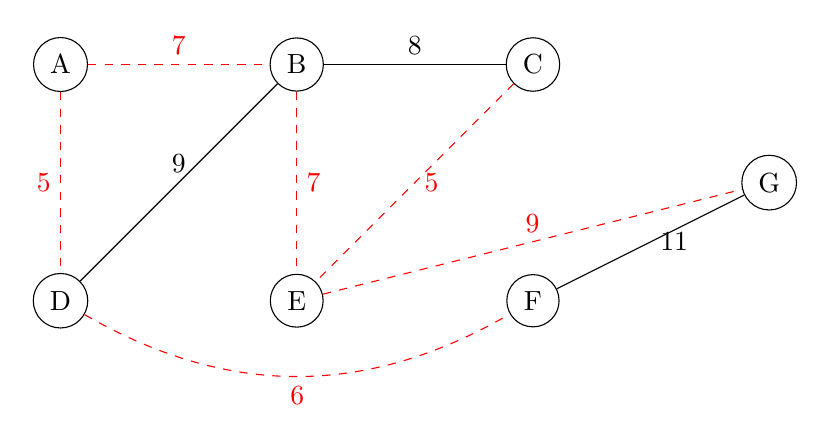
\begin{tikzpicture}
  \node[shape=circle,draw=black] (a) at (0,0) {A};
  \node[shape=circle,draw=black] (b) at (3,0) {B};
  \node[shape=circle,draw=black] (c) at (6,0) {C};
  \node[shape=circle,draw=black] (d) at (0,-3) {D};
  \node[shape=circle,draw=black] (e) at (3,-3) {E};
  \node[shape=circle,draw=black] (f) at (6,-3) {F};
  \node[shape=circle,draw=black] (g) at (9,-1.5) {G};
  \path [-,red,dashed](a) edge node[above] {7} (b);
  \path [-,red,dashed](b) edge node[right] {7} (e);
  \path [-,red,dashed](e) edge node[above] {9} (g);
  \path [-,red,dashed](d) edge[bend right=30] node[below] {6} (f);
  \path [-,red,dashed](a) edge node[left] {5} (d);
  \path [-](b) edge node[above] {8} (c);
  \path [-](b) edge node[above] {9} (d);
  \path [-,red,dashed](c) edge node[right] {5} (e);
  \path [-](f) edge node[right] {11} (g);
\end{tikzpicture}
